% 2-15-rb-tree.tex

%%%%%%%%%%%%%%%%%%%%
\documentclass[a4paper, justified]{tufte-handout}

% hw-preamble.tex

% geometry for A4 paper
% See https://tex.stackexchange.com/a/119912/23098
\geometry{
  left=20.0mm,
  top=20.0mm,
  bottom=20.0mm,
  textwidth=130mm, % main text block
  marginparsep=5.0mm, % gutter between main text block and margin notes
  marginparwidth=50.0mm % width of margin notes
}

% for colors
\usepackage{xcolor} % usage: \color{red}{text}
% predefined colors
\newcommand{\red}[1]{\textcolor{red}{#1}} % usage: \red{text}
\newcommand{\blue}[1]{\textcolor{blue}{#1}}
\newcommand{\teal}[1]{\textcolor{teal}{#1}}

\usepackage{todonotes}

% heading
\usepackage{sectsty}
\setcounter{secnumdepth}{2}
\allsectionsfont{\centering\huge\rmfamily}

% for Chinese
\usepackage{xeCJK}
\usepackage{zhnumber}
\setCJKmainfont[BoldFont=FandolSong-Bold.otf]{FandolSong-Regular.otf}

% for fonts
\usepackage{fontspec}
\newcommand{\song}{\CJKfamily{song}} 
\newcommand{\kai}{\CJKfamily{kai}} 

% To fix the ``MakeTextLowerCase'' bug:
% See https://github.com/Tufte-LaTeX/tufte-latex/issues/64#issuecomment-78572017
% Set up the spacing using fontspec features
\renewcommand\allcapsspacing[1]{{\addfontfeature{LetterSpace=15}#1}}
\renewcommand\smallcapsspacing[1]{{\addfontfeature{LetterSpace=10}#1}}

% for url
\usepackage{hyperref}
\hypersetup{colorlinks = true, 
  linkcolor = teal,
  urlcolor  = teal,
  citecolor = blue,
  anchorcolor = blue}

\newcommand{\me}[4]{
    \author{
      {\bfseries 姓名:}\underline{#1}\hspace{2em}
      {\bfseries 学号:}\underline{#2}\hspace{2em}\\[10pt]
      {\bfseries 评分:}\underline{#3\hspace{3em}}\hspace{2em}
      {\bfseries 评阅:}\underline{#4\hspace{3em}}
  }
}

% Please ALWAYS Keep This.
\newcommand{\noplagiarism}{
  \begin{center}
    \fbox{\begin{tabular}{@{}c@{}}
      请独立完成作业,不得抄袭。\\
      若得到他人帮助, 请致谢。\\
      若参考了其它资料,请给出引用。\\
      鼓励讨论,但需独立书写解题过程。
    \end{tabular}}
  \end{center}
}

\newcommand{\goal}[1]{
  \begin{center}{\fcolorbox{blue}{yellow!60}{\parbox{0.50\textwidth}{\large 
    \begin{itemize}
      \item 体会``思维的乐趣''
      \item 初步了解递归与数学归纳法 
      \item 初步接触算法概念与问题下界概念
    \end{itemize}}}}
  \end{center}
}

% Each hw consists of four parts:
\newcommand{\beginrequired}{\hspace{5em}\section{作业 (必做部分)}}
\newcommand{\beginoptional}{\section{作业 (选做部分)}}
\newcommand{\beginot}{\section{Open Topics}}
\newcommand{\begincorrection}{\section{订正}}
\newcommand{\beginfb}{\section{反馈}}

% for math
\usepackage{amsmath, mathtools, amsfonts, amssymb}
\newcommand{\set}[1]{\{#1\}}

% define theorem-like environments
\usepackage[amsmath, thmmarks]{ntheorem}

\theoremstyle{break}
\theorempreskip{2.0\topsep}
\theorembodyfont{\song}
\theoremseparator{}
\newtheorem{problem}{题目}[subsection]
\renewcommand{\theproblem}{\arabic{problem}}
\newtheorem{ot}{Open Topics}

\theorempreskip{3.0\topsep}
\theoremheaderfont{\kai\bfseries}
\theoremseparator{:}
\theorempostwork{\bigskip\hrule}
\newtheorem*{solution}{解答}
\theorempostwork{\bigskip\hrule}
\newtheorem*{revision}{订正}

\theoremstyle{plain}
\newtheorem*{cause}{错因分析}
\newtheorem*{remark}{注}

\theoremstyle{break}
\theorempostwork{\bigskip\hrule}
\theoremsymbol{\ensuremath{\Box}}
\newtheorem*{proof}{证明}

% \newcommand{\ot}{\blue{\bf [OT]}}

% for figs
\renewcommand\figurename{图}
\renewcommand\tablename{表}

% for fig without caption: #1: width/size; #2: fig file
\newcommand{\fig}[2]{
  \begin{figure}[htbp]
    \centering
    \includegraphics[#1]{#2}
  \end{figure}
}
% for fig with caption: #1: width/size; #2: fig file; #3: caption
\newcommand{\figcap}[3]{
  \begin{figure}[htbp]
    \centering
    \includegraphics[#1]{#2}
    \caption{#3}
  \end{figure}
}
% for fig with both caption and label: #1: width/size; #2: fig file; #3: caption; #4: label
\newcommand{\figcaplbl}[4]{
  \begin{figure}[htbp]
    \centering
    \includegraphics[#1]{#2}
    \caption{#3}
    \label{#4}
  \end{figure}
}
% for margin fig without caption: #1: width/size; #2: fig file
\newcommand{\mfig}[2]{
  \begin{marginfigure}
    \centering
    \includegraphics[#1]{#2}
  \end{marginfigure}
}
% for margin fig with caption: #1: width/size; #2: fig file; #3: caption
\newcommand{\mfigcap}[3]{
  \begin{marginfigure}
    \centering
    \includegraphics[#1]{#2}
    \caption{#3}
  \end{marginfigure}
}

\usepackage{fancyvrb}

% for algorithms
\usepackage[]{algorithm}
\usepackage[]{algpseudocode} % noend
% See [Adjust the indentation whithin the algorithmicx-package when a line is broken](https://tex.stackexchange.com/a/68540/23098)
\newcommand{\algparbox}[1]{\parbox[t]{\dimexpr\linewidth-\algorithmicindent}{#1\strut}}
\newcommand{\hStatex}[0]{\vspace{5pt}}
\makeatletter
\newlength{\trianglerightwidth}
\settowidth{\trianglerightwidth}{$\triangleright$~}
\algnewcommand{\LineComment}[1]{\Statex \hskip\ALG@thistlm \(\triangleright\) #1}
\algnewcommand{\LineCommentCont}[1]{\Statex \hskip\ALG@thistlm%
  \parbox[t]{\dimexpr\linewidth-\ALG@thistlm}{\hangindent=\trianglerightwidth \hangafter=1 \strut$\triangleright$ #1\strut}}
\makeatother

% for footnote/marginnote
% see https://tex.stackexchange.com/a/133265/23098
\usepackage{tikz}
\newcommand{\circled}[1]{%
  \tikz[baseline=(char.base)]
  \node [draw, circle, inner sep = 0.5pt, font = \tiny, minimum size = 8pt] (char) {#1};
}
\renewcommand\thefootnote{\protect\circled{\arabic{footnote}}} % feel free to modify this file
%%%%%%%%%%%%%%%%%%%%
\title{第4-1讲: 群论初步}
\me{朱宇博}{191220186 }{}{}
\date{\zhtoday} % or like 2019年9月13日
%%%%%%%%%%%%%%%%%%%%
\begin{document}
\maketitle
%%%%%%%%%%%%%%%%%%%%
\noplagiarism % always keep this line
%%%%%%%%%%%%%%%%%%%%
\begin{abstract}
  % \begin{center}{\fcolorbox{blue}{yellow!60}{\parbox{0.65\textwidth}{\large 
  %   \begin{itemize}
  %     \item 
  %   \end{itemize}}}}
  % \end{center}
\end{abstract}
%%%%%%%%%%%%%%%%%%%%
\beginrequired

%%%%%%%%%%%%%%%
\begin{problem}[TJ 3-3]
\end{problem}

\begin{solution}
 \begin{figure}[htbp]
    \centering
    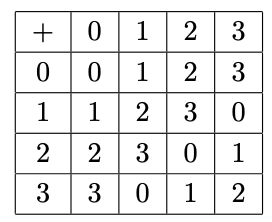
\includegraphics[width = 0.30\linewidth]{figs/a}
  \end{figure}
   \begin{figure}[htbp]
    \centering
    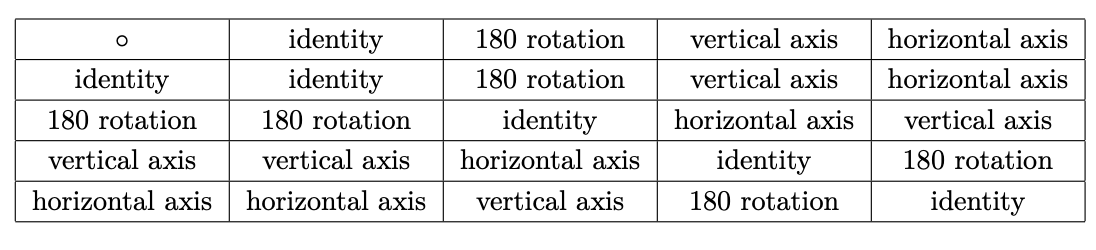
\includegraphics[width = 0.90\linewidth]{figs/b}
  \end{figure}

\noindent $\mathbb{Z}_4$  has $1$ nontrivial proper subset $\{0,2\}$. The number of other group's nontrivial proper is more than one. So they are not same group.  
\end{solution}
%%%%%%%%%%%%%%%

%%%%%%%%%%%%%%%
\begin{problem}[TJ-3-7]
\end{problem}

\begin{solution}
(1)associative law:\\
\[
(a* b) * c = (ab+a+b)*c=a+b+c+ab+ac+bc+ab+abc=a*(bc+b+c)=a*(b*c)
\]
(2)identity element:\\
\[
\forall x\in R\backslash \{-1\},x*0=x
\]
(3)inverse element:\\
\[
\forall x\in R\backslash \{-1\},\exists y = -\frac{a}{a+1}\in R\backslash \{-1\},st. a*b=0
\]
(4)abelian:\\
\[
a*b=a+b+ab=b*a 
\]
\end{solution}
%%%%%%%%%%%%%%%

%%%%%%%%%%%%%%%
\begin{problem}[TJ 3-39]
\end{problem}

\begin{solution}
\[
\forall a=x+yi, b=m+ni\in \mathbb{T}, ab^{-1}=(x+yi)(m-ni)=xm+yn+(my-nx)i\in \mathbb{T}
\]
So $\mathbb{T}$ is a subgroup of $\mathbb{C^*}$
\end{solution}
%%%%%%%%%%%%%%%

%%%%%%%%%%%%%%%
\begin{problem}[TJ 3-42]
\end{problem}

\begin{solution}
$\forall g,h\in H$, Let
\[
g=\begin{pmatrix}
    a_1 & b_1\\\\
    c_1 & d_1 \\\\
 \end{pmatrix}
\qquad h = \begin{pmatrix}
    a_2 & b_2 \\\\
    c_2 & d_2 \\\\
\end{pmatrix}
\]
We have that
\[
h^{-1}=  \begin{pmatrix}
    -a_2 & -b_2 \\\\
    -c_2 & -d_2 \\\\
\end{pmatrix}
\qquad g\circ h^{-1} = \begin{pmatrix}
    a_1-a_2 & b_1-b_2 \\\\
    c_1-c_2 & d_1-d_2 \\\\
\end{pmatrix}
\]
So $g\circ h^{-1}\in H$, $H$ is a subgroup of $G$.
\end{solution}
%%%%%%%%%%%%%%%

%%%%%%%%%%%%%%%
\begin{problem}[TJ 3-49]
\end{problem}

\begin{solution}
\[
a^4b=a^3ab=eab=ab=ba
\]
\end{solution}
%%%%%%%%%%%%%%%

%%%%%%%%%%%%%%%
\begin{problem}[TJ 3-51]
\end{problem}

\begin{solution}
\[
\forall x\in G, xe=x=x^{-1}e^{-1}=x^{-1}
\]
\[
\to \forall x,y\in G, xy\in G, xy=(xy)^{-1}=(y^{-1}x^{-1})=yx\\
\]
So the group $G$ is abelian.
\end{solution}
%%%%%%%%%%%%%%%

%%%%%%%%%%%%%%%
\begin{problem}[TJ 4-1]
\end{problem}

\begin{solution}
(a)\\
False. $49$ is a generator of $\mathbb{Z}_{60}$, but it is not prime.\\
(b)\\
False. $1,3,5,7$ are all not generator of $U(8)$.\\
(c)\\
False. Assume that g is a generator of $\mathbb{Q}$, but $g$ can not generate $\frac{g}{2}$.\\
(d)\\
False. The symmetry group of an equilateral triangle $S3$ is not cyclic, but the subgroup of $S3$ are all cyclic.\\
(e)\\
True. \\
Suppose, to the contrary, an infinite group $G$ has finite number of subgroup.\\
(1) If $G$ has an infinite order  generator $g$, then $<g>, <g^2>, <g^3>, <g^4>,...,<g^k>$ are all the subgroup of $G$, so it has infinite number of subgroup. It is contradict with the assumption.\\
(2) If the order of generators are all finite, then we let S = $\{<x>|x\in G\}$. We have that $S$ is a finite set. The group $G$ is the union of the finite set $S$, so $G$ is finite, it is contradict with the assumption.\\
Therefore, a group with a finite number of subgroups is finite.
\end{solution}
%%%%%%%%%%%%%%%

%%%%%%%%%%%%%%%
\begin{problem}[TJ 4-24]
\end{problem}

\begin{solution}
$\phi(pq)=\phi(p)\phi(q)=(p-1)(q-1)=pq-p-q+1$(p and q are different primes)
\end{solution}
%%%%%%%%%%%%%%%




%%%%%%%%%%%%%%%
\begin{problem}[TJ 4-12]
\end{problem}

\begin{solution}
one generator: $\mathbb{Z}_2$\\
Two generators: $\mathbb{Z}_4$\\
Four generators: $\mathbb{Z}_8$\\
$n$ generators: $\exists x, st. \phi(x)=n$. $\mathbb{Z}_{x}$ has $n$ generators.
\end{solution}
%%%%%%%%%%%%%%%

%%%%%%%%%%%%%%%
\begin{problem}[TJ 4-32]
\end{problem}

\begin{solution}
Due to Theorem4.13 in TJ, $y=x^{k}$, the order of $y$ is $\frac{n}{gcd(k,n)}=\frac{n}{1}=n$. Therefore, $y$ is a generator of $G$.
\end{solution}
%%%%%%%%%%%%%%%

%%%%%%%%%%%%%%%%%%%%
\beginoptional

%%%%%%%%%%%%%%%
\begin{problem}[$Z_p$]
证明:设$p$为素数,则$Z_p=\{1,2,...,p-1\}$关于$p$\textbf{乘法}构成的$p-1$阶循环群。(此处的$1,2,...,p-1$是模$p$等价类的代表元)
\end{problem}

\begin{solution}
\end{solution}
%%%%%%%%%%%%%%%

%%%%%%%%%%%%%%%
\begin{problem}[SageMath学习]
安装 \href{https://www.sagemath.org/}{SageMath},并学习 TJ 第三章 3.6节、3.7节; 第四章 4.6节、4.7节 关于 SageMath 的内容
\end{problem}

\begin{solution}
\end{solution}
%%%%%%%%%%%%%%%

%%%%%%%%%%%%%%%%%%%%
\beginot
%%%%%%%%%%%%%%%
\fig{ }{figs/mobile-group-demo.png}

在二维平面上的``移动''(例如向东北30度移动9公里)。
	你能够以这些``移动''为元素构建一个群吗?
\begin{ot}[``移动''群-1]	
	\begin{itemize}
	\item 它的几何元素和运算分别是什么?
	\item 它为什么符合群的定义?
	\item 它是阿贝尔群吗?为什么?
	\end{itemize}
\end{ot}

% \begin{solution}
% \end{solution}
%%%%%%%%%%%%%%%

%%%%%%%%%%%%%%%
\begin{ot}[``移动''群-2]	
	\begin{itemize}
	\item 你能找出它的一些子群吗?并说明为什么找到的是子群
	\item 它是循环群吗?如果是,生成元是什么?生成元唯一吗?如果不是,如何改造出一个循环群?
	\item 你能找出这个(改造后的)循环群的一些子群么?它们是循环群么?
	\end{itemize}
\end{ot}


% \begin{solution}
% \end{solution}
%%%%%%%%%%%%%%%


% \vspace{0.50cm}
%%%%%%%%%%%%%%%
% \begin{ot}[]
% 
%   \noindent 参考资料:
%   \begin{itemize}
%     \item 
%   \end{itemize}
% \end{ot}

% \begin{solution}
% \end{solution}
%%%%%%%%%%%%%%%

%%%%%%%%%%%%%%%%%%%%
% 如果没有需要订正的题目,可以把这部分删掉

% \begincorrection
%%%%%%%%%%%%%%%%%%%%

%%%%%%%%%%%%%%%%%%%%
% 如果没有反馈,可以把这部分删掉
\beginfb

% 你可以写
% ~\footnote{优先推荐 \href{problemoverflow.top}{ProblemOverflow}}:
% \begin{itemize}
%   \item 对课程及教师的建议与意见
%   \item 教材中不理解的内容
%   \item 希望深入了解的内容
%   \item $\cdots$
% \end{itemize}
%%%%%%%%%%%%%%%%%%%%
% \bibliography{2-5-solving-recurrence}
% \bibliographystyle{plainnat}
%%%%%%%%%%%%%%%%%%%%
\end{document}